\documentclass[a4paper]{article}
\usepackage[ngerman]{babel}
\usepackage{amsthm}
\usepackage{amsmath}
\usepackage{amsfonts}
\usepackage{parskip}
\usepackage{graphicx}
\usepackage{color}
\usepackage{listings}

\usepackage{color}

\definecolor{mygreen}{rgb}{0,0.6,0}
\definecolor{mygray}{rgb}{0.5,0.5,0.5}
\definecolor{mymauve}{rgb}{0.58,0,0.82}

\lstset{ 
  backgroundcolor=\color{white},
  basicstyle=\footnotesize,
  breakatwhitespace=false,
  breaklines=true,
  captionpos=b,
  commentstyle=\color{mygreen},
  extendedchars=true,
  frame=single,
  keepspaces=true,
  keywordstyle=\color{blue},
  language=Java,
  numbers=left,
  numbersep=5pt,
  numberstyle=\color{mygray},
  rulecolor=\color{black},
  showspaces=false,
  showstringspaces=false,
  showtabs=false,
  stepnumber=5,
  stringstyle=\color{mymauve},
  tabsize=2,
  title=\lstname
}

\pagestyle{headings}

\newtheorem{satz}{Satz}
\theoremstyle{definition}
\newtheorem{definition}{Definition}

\title{Dokumentation}
\author{
    Matthias Vonend
    \and
    Jan Grübener
    \and
    Patrick Mischka
    \and
    Michael Angermeier
    \and
    Troy Keßler
    \and
    Aaron Schweig
    \and
}

\begin{document}

    \maketitle
    \tableofcontents

    % oder clearpage
    \vspace{0.2cm}

    % TODO add information about git

    \section{Basisanforderungen}
        % !TEX root = ./docs.tex




\begin{figure}[h]
    \centering
    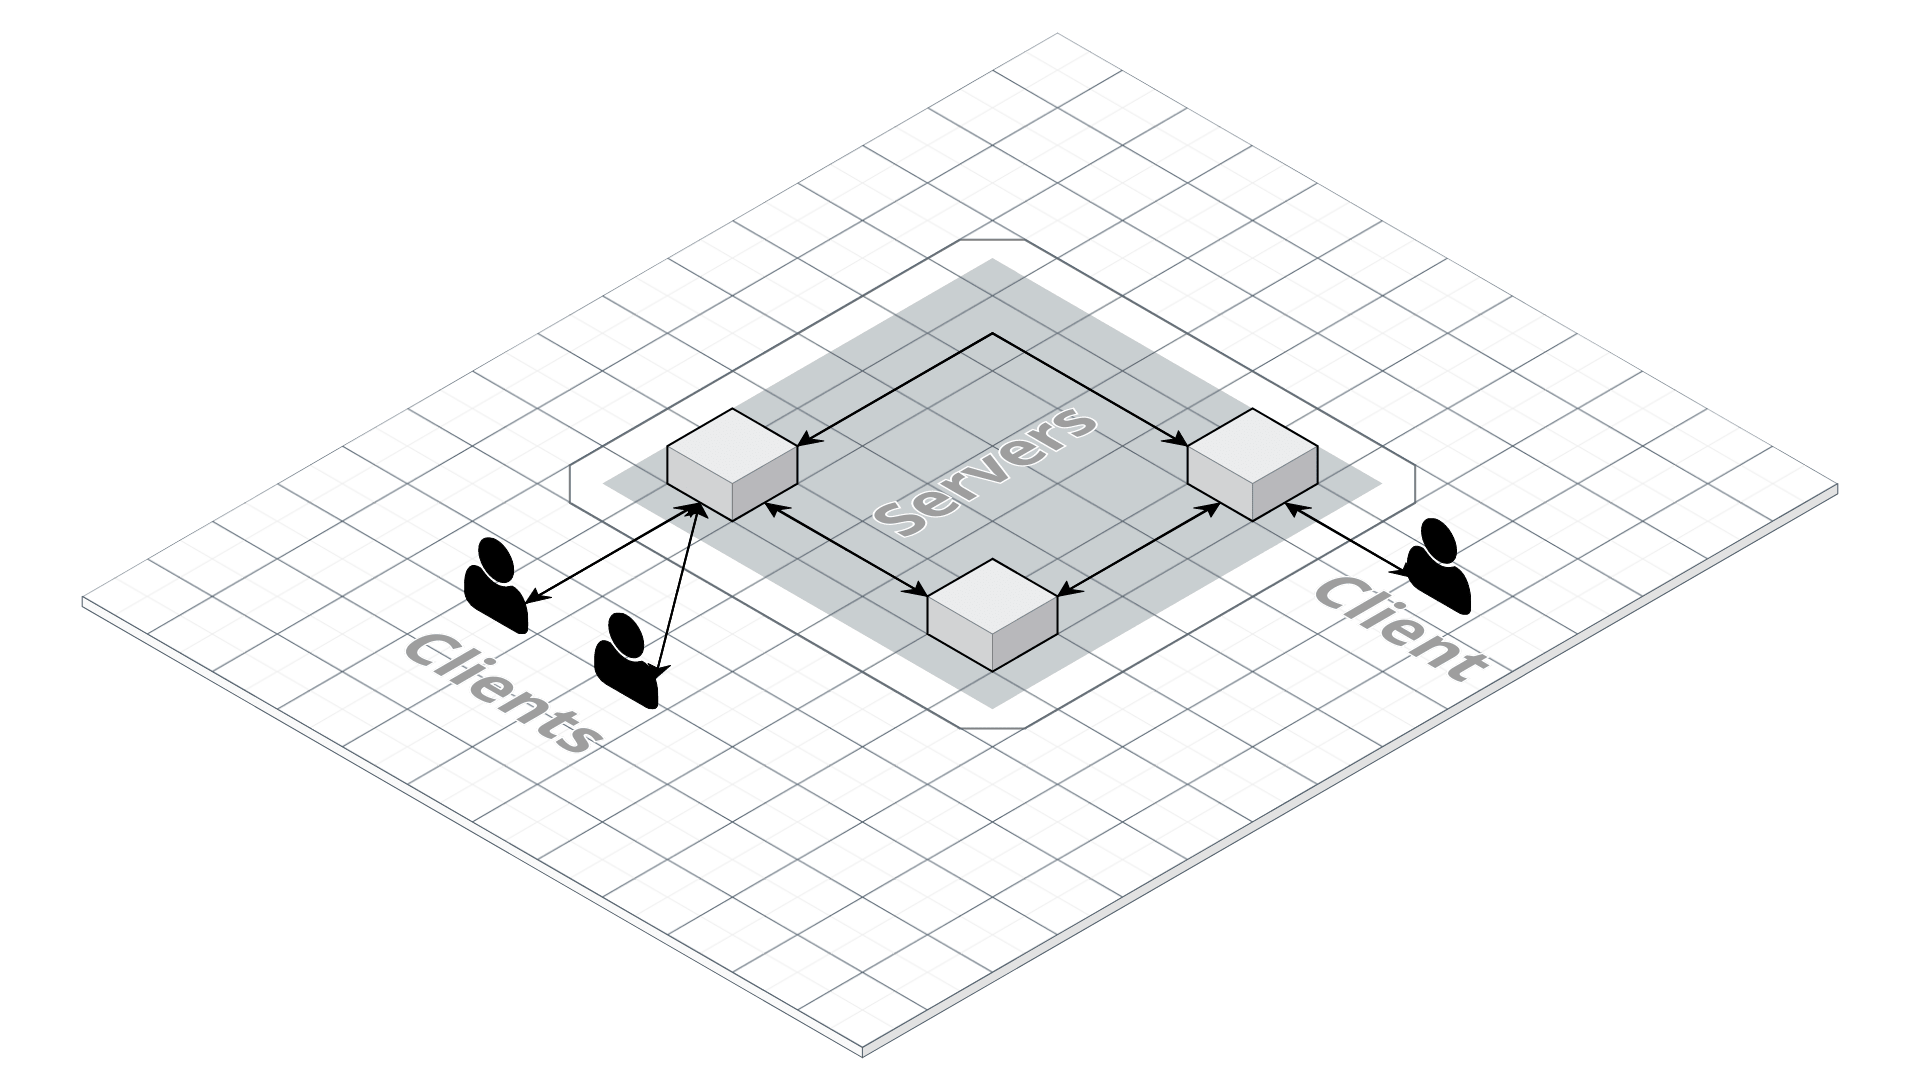
\includegraphics[width=\textwidth]{architecture.png}
    
    \caption{Architektur}
    \label{}
\end{figure}

\subsection{Chatfunktionalität}
Damit ein Chat ablaufen kann muss zunächst eine Verbindung zu einem Server aufgebaut werden. Dazu wählt der Client zunächst einen zufälligen Server aus und versucht sich zu verbinden. Wurde eine Verbindung erfolgreich aufgebaut, kann sich der Nutzer mit seinem Nutzername und seinem Password anmelden. Sobald der Nutzer angemeldet ist sendet der Server ihm alle benötigten Informationen inklusiver der verpassten Nachrichten. Jede Nachricht hat eine Datum wann es erstmalig an einem Server eingetroffen ist. Anhand von diesem werden die Nachrichten sortiert, damit der Client die korrekte Reihenfolge darstellen kann.

Möchte dieser eine Nachricht an einen weiteren Client senden, schickt er diese an seine verbundene Node und überlässt die Zustellung dieser. Da alle Nachrichten aus Persistenzgründen an alle Nodes verteilt werden müssen, brauchen die Nodes keine Information über die Clients anderer Nodes. Im Falle einer solchen Anforderung (z.\,B. Abfrage ob ein anderer Nutzer aktiv ist) könnte ein Protokoll ähnlich zu Routing-Tabellen implementiert werden. Empfängt eine Node eine Nachricht, egal ob von einem Client oder von einer anderen Node, überprüft diese ob die Nachricht für einen ihr bekannten Client bestimmt war und sendet diese gegebenenfalls an diesen.

//TODO Nach einer erfolgreichen Anmeldung kann der Nutzer
// create chat und so bla :)


\subsection{Fehlerbehandlung}
Aus den Anforderungen geht hervor, dass es mindestens zwei Server geben muss, die sämtliche Informationen des Chatsystems besitzen müssen. Bricht eine Node zusammen muss dementsprechend eine andere Node dessen Aufgabe übernehmen.
\subsubsection{Client}
//TODO Troy

Im Fehlerfall scheitert das Senden einer Nachricht an den Server. In diesem Fall versucht sich der Client mit einer anderen Node zu verbinden und sendet die Nachricht erneut.

\subsubsection{Server}
Serverseitig können verschiedene Fehler auftretten. VIele Fehler werden bereits durch das TCP-Protokoll verhindert. Dennoch können grundsätzlich die folgende Fehlerfälle eintretten:
\begin{enumerate}
    \item Nachricht des Clients kann nicht korrekt empfangen/gesendet werden\\
        In diesem Fall muss der Server davon ausgehen, dass die Verbindung zusammengebrochen ist und er beendet seine Verbindung. Der Server verlässt sich darauf, dass der Client erneut eine Verbindung aufbaut. Alle für den Client relevanten Nachrichten werden dann zu diesem übertragen und der Client muss neue Informationen zurück übertragen
    \item Nachrichten einer Nachbarnode können nicht korrekt empfangen/gesendet werden\\
        Ähnlich zur Clientverbindung muss der Server davon ausgehen dass die Verbindung zusammengebrochen ist. Allerdings ist der Server hier selbst dafür zuständig sich erneut zu verbinden. Sämtliche Nachrichten, die an eine Node gesendet werden müssen werden in einer Queue aufbewahrt und nacheinander gesendet. Scheitert die Verbindung, so bleibt die Queue unverändert und wird nach einem erneuten Verbinden weiter abgearbeitet. Es wird solange versucht zu verbinden, bis eine Verbindung zustande gekommen ist. Sobald eine Verbindung wieder aufgebaut wurde synchronisieren sich die Nodes um wieder einen vollständigen Informationsstand zu besitzen.
        Sind keine Nachrichten zu senden hat die Node keine Möglichkeit festzustellen ob eine Verbindung noch existiert. Zu diesem Zweck existiert ein Heartbeat, der periodisch die Nachbarnodes anpingt und so prüft ob die Verbindung noch existiert.
\end{enumerate}
Wie gerade beschrieben führen alle beteiligten stehts eine synchronisation durch wodurch diese immer den kompletten Informationsbestand besitzen.

Eine Veränderung des Datenbestandes muss dem entsprechend an alle anderen Nodes weiter gegeben werden. Dadurch sind alle Server gleichwertige Servern.





    \section{Erweiterungen}
        % !TEX root = ./docs.tex

\subsection{Grafische Oberfläche bei den Nutzern}

\subsection{Verwendung von Emojis}

\subsection{Mehrere Chatverläufe pro Nutzer}

\subsection{Persistentes Speichern der Chatverläufe}

\subsection{Verschlüsselte serverseitige Speicherung der Chats}

\subsection{Gruppenchats}

\subsection{Verschlüsselte Übertragung der Chat-Nachrichten}

%\subsection{3 replizierte Server mit Majority Consensus Strategie}
% Gibt in unserem Ansatz keinen Sinn


    \clearpage
    \section{Anhang}
        % !TEX root = ./docs.tex



\lstinputlisting[linerange={37-76}, firstnumber=37]{../src/main/java/vs/chat/server/ConnectionHandler.java}
 % Per section? -> problematic ref


    \section{TODOS}
        Das doc schreiben duh :P
        Konfliktvermeidung ansprechen -> Datenbanken vergleich mit UUID als Fremdschlüssel
        UUIDs erwähnen
        Code walkthrough + kommentieren
        Titlepage überarbeiten

\end{document}